\documentclass[conference]{IEEEtran}

\usepackage[utf8]{inputenc}
\usepackage{amsmath}
\usepackage{graphicx}
\usepackage{tabularx}
\usepackage{adjustbox}
%\usepackage[colorinlistoftodos]{todonotes}
\usepackage{csquotes}
\usepackage{comment}
\usepackage{imakeidx}
%tabela
\usepackage{multirow}
\usepackage{xcolor}
\usepackage[margin=2.5cm]{geometry}
\usepackage{hyperref} %to show links
\usepackage{titling}
\usepackage[ddmmyyyy]{datetime}
\usepackage{setspace}
\usepackage{indentfirst}

%to define placement of tables and images in strict mode
%\usepackage{placeins}

\usepackage[style=ieee]{biblatex} 
\addbibresource{ref.bib}
\input{vars}
\linespread{1.2}

\bibliography{sources}

\begin{document}

\title{Implementing an HTML5 mobile simulation utilizing web workers}

\author{authored by\\
        Lari Alakukku (528362),
        Miika Rouvinen (356770),
        Ilkka Malassu (430463)}%

\makeatletter         
\def\@maketitle{
\begin{center}
{\Huge \bfseries \sffamily \@title }\\[4ex] 
Submitted on \@date\\
{\normalsize \@author}\\[4ex] 
%\@date\\[8ex]
\end{center}}
\makeatother


% make the title area
\maketitle

\begin{IEEEkeywords}
HTML5, web, workers
\end{IEEEkeywords}

%%%%%%%%%%%%%%%%%%%%%%%%%%%%%%%%%%%%%%%%%%%%%%%%%%%%%  
\begin{abstract}

Abstract of the paper here
 
\end{abstract}

\section{Introduction}
\label{chap:introduction}

The internet has progressed from a distributed document sharing system to a platform that can host computationally demanding applications. This evolution makes performance a crucial web-client requirement. The modern browser provides a possibility to develop intricate web applications utilizing only HTML, CSS and JavaScript. The developers of a web-based game, for example, need to optimize their code taking the processing capability of different browsers into account. Current hardware mostly focuses on concurrent execution while many web applications still only use the main browser thread. HTML5 introduced web workers as a first step towards concurrent execution in web applications. \cite{doha}

Web workers offload processing tasks from the main browser thread to background worker threads, requiring the platform to have basic support for concurrency. The communication between the threads is facilitated with message sending. Web workers can not use DOM operations or access window objects and parent objects. Also, direct data sharing between the main thread and the worker threads is not possible. \cite{doha, watanabe}


\section{Related Work}
\label{sec:soa}

For web-based games, Erbad et al. \cite{doha} propose a concurrent processing solution called DOHA, which consists of game event-loops running in worker threads and MultiProc, which is the module for scheduling, state management and other concurrent execution related tasks. Their game implementation had three main components: simulation, graphics rendering and AI. The main thread handles rendering and offloads game event processing to web workers. This communication also requires the sending of state information. In general, DOHA offered better scalability and responsiveness across different platforms. However, thread communication required replicating state across workers, which increased jitter.
Zhang et al. \cite{zhang} introduce WWOF, which is a framework for seamlessly offloading web workers to the cloud. On average, the framework achieved energy savings of 85\% on devices such as mobile phones, desktop computers and pads. The performance of the devices improved by a factor of 2-4.
Verdú et al. \cite{verdu} examine how utilizing web workers scales the performance of a JavaScript application. They found that the optimal number of workers depends on various factors such as the CPU architecture and the browser. Using a large number of web workers did not prove to be beneficial compared to using only a few.

\section{Implementation}

Here we present our implementation.

\subsection{Context} 
\label{sec:context}

Maybe a subsection if needed.

%%%%%%%%%%%%%%%%%%%%%%%%%%%%%%%%%%%%%%%%%%%%%%%%%%%%%  
\section{Evaluation}
\label{sec:sec2}

Here we present our evaluation of the implementation.
Example results in Figure \ref{fig:labeloffigure}. 

\begin{figure}[ht]
	\centering
	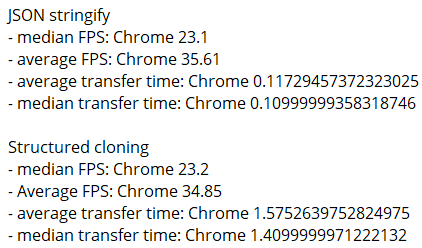
\includegraphics[scale=0.5]{figs/example.png}
	\caption{This is a figure}
	\label{fig:labeloffigure}
\end{figure}

\section{Conclusions}
\label{sec:conc}

We conclude our research paper here.

\printbibliography[title={References}]

\end{document}